\section{Introduction}

%0. Abstract
%	1. 建立了一个 UAV-BD 的数据集
%	2. 比较 Faster RCNN, SSD, RRPN, DRBox 算法
%
%1. Introduction
%	1. 建立这个数据集的动机(目的) -> 旅游景区垃圾丛生, 传统人力回收的方式过于危险, 可以使用无人机辅助定位并捡垃圾, 减少工人危险系数 -> 为了实现无人机定位瓶子, 需要检测瓶子 -> 引出数据集
%	
%	2. 无人机的发展, 无人机的特性, 对数据集的影响 -> 引出无人机视角下, 目标的外形与 PASCAL VOC, COCO 等数据集完全不同, 不能使用当前公开的数据集训练模型 (数据的重要性) -> 引出无人机视角下瓶子的特性
%	
%	3. 无人机视角下瓶子的特性 -> (1) 尺寸小, (2) 尺度变化大, (3) 种类多, (4) 具有旋转性, (5) 透明特性, (6) 背景复杂 -> 引出我们建立了 UAV-Bottle Dataset (UAV-DB) 数据集 -> 数据集展示 (一张大图, 下面三张小图)
%	
%	4. 目标检测算法的发展 -> 简要概括传统目标检测算法, 主要是 RCNN, Faster RCNN, Faster RCNN 线和 YOLO SSD 线 -> 发现瓶子旋转特性对模型影响很大, 引出 RRPN 和 DRBox 
%	
%2. UAV-Bottle Dataset
%	1. 无人机视角下数据集特性分析 -> 引出数据集收集和构建方式的合理性 -> (1) 尺寸小(裁剪成小图, 使用具有多尺度特性的算法作为 pipline), (2) 尺度变化大(无人机在不同飞行高度下采集图像, 10m-50m), (3) 种类多(使用尽量多种类的饮料瓶), (4) 具有旋转性(旋转标注, 介绍优点, 并指出传统标注方式的缺点(图示), 使用能使用 RBox 作为 pipline), (5) 透明特性, 训练难度大(选择透明性较好的瓶子), (6) 背景复杂(选择可能出现的场景收集数据, 分为8个场景, 并分类存储, 方便算法针对特定场景进行优化, 展示不同场景下的图像) -> 引出收集方式
%	
%	2. 收集方式 -> 两阶段收集, 无人机飞行高度, 瓶子种类, 背景分类 (展示不同背景下的瓶子), 裁剪方式, 图片大小, 如何处理边界图像
%	
%	3. 数量统计 -> 分场景统计 (1) 大图数量 (2) 小图数量 (3) 大图中目标数量 (4) 小图中目标数量 (5) Scale Angle Ratio 分布特性 (6) train val test 如何划分 (1-4表格展示, 5直方图展示)
%	4. 标注方式 -> 使用旋转框进行标注, 用于训练 RRPN 和 DRBox 等能使用旋转框训练的算法, 对旋转框做最小外接矩形变成传统框(图示), 用于训练传统算法
%
%3. Pipline Experiments and Result
%	1. 使用本数据集训练了四种基于深度学习的算法 Faster RCNN, SSD, RRPN, DRBox
%	2. Faster RCNN 和 SSD 使用原版参数
%	3. 简要介绍 RRPN 和 DRBox 在 Faster RCNN 和 SSD 算法上的改进, 他们如何使用旋转标注框 (画出pipline)
%	4. 针对 UAV-BD 对 RRPN 和 DRBox 的改进 -> (1) 根据 UAB-BD 的数据分布修改了 RRPN 的 Rotation Anchor, (2) 根据 UAV-BD 的数据分布修改了 DRBox 的 prior box
%	5. 对比四种深度学习算法的 PR 曲线和 AP 性能, 给出简要结论 -> 旋转bbox能提高算法的性能
%
%
%4. Conclusion
%	1. 我们建立了 UAV-BD 数据集, 并将公开这个数据集
%	
%	2. 我们使用本数据集训练了 Faster RCNN, SSD, RRPN, DRBox, 并比较了他们之间的性能差异, 得出旋转标注对模型训练具有一定优势
%
%5. Reference


\label{sec:intro}

%% 1. 建立本数据集的动机和目的

Nowadays, with the popularity of tourist attractions, there is a lot of rubbish, especially bottles, need to recycle. However, these bottles are mainly collected by human observation, which is time-consuming, laborious and dangerous. In order to solve these problems, we use the unmanned aerial vehicle (UAV) to locate and even recycle bottles. We also build a UAV bottle dataset (UAV-BD) to locate bottles more effectively.


%% 2. UAV 的发展, 拍摄图像的特性, 对目标检测的影响 -> 引出无人机视角下瓶子的特性

Detecting objects in UAV images plays an important role in many applications and has received significant attention in recent years\cite{UAV2}. However, it is still a challenging problem due to the high resolution with the extremely high level of detail, various shooting platform, limited annotated data, and limited processing time for real-time applications\cite{car_detection}. In UAV images, the bottle looks completely different from the bottle in datasets such as PASCAL VOC\cite{PASCALVOC}, Microsoft COCO\cite{COCO}, etc. The difference between PASCAL VOC and our dataset is shown in Fig.\ref{bottle_VOC_UAV}.

\begin{figure}
	\centering
	\subfigure[Bottles in PASCAL VOC]
	{
		\label{bottle_VOC}
		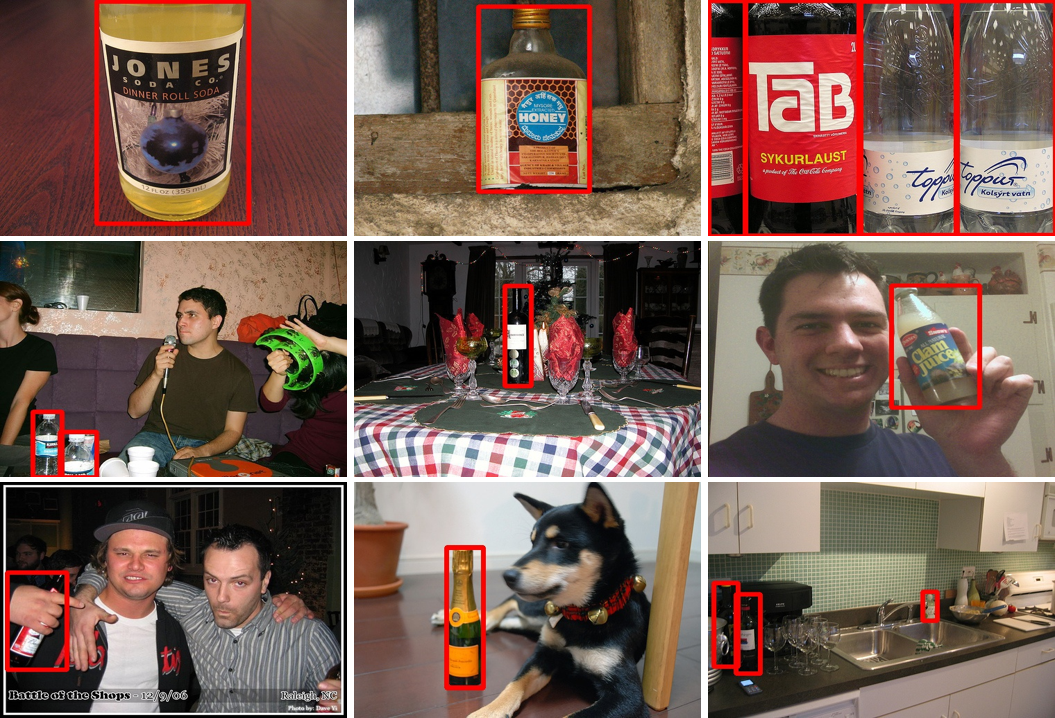
\includegraphics[height=0.37\linewidth]{images/bottle_VOC.png}
	}
	\subfigure[Bottles in UAV images]
	{
		\label{bottle_UAV}
		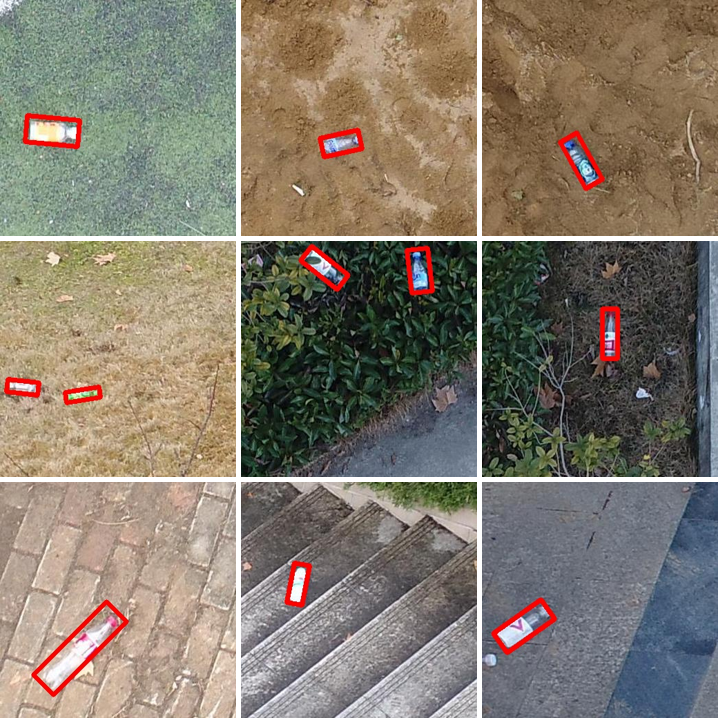
\includegraphics[height=0.37\linewidth]{images/bottle_UAV.png}
	}
	
	\caption{Comparison of bottles in PASCAL VOC dataset and UAV images}
	\label{bottle_VOC_UAV}
\end{figure}

%% 3. 无人机视角下瓶子的特性

As to UAV images, detecting bottles exists several unique challenges. First, the size of bottles is very small, which is generally less than $ 50\times 50 $ pixels. At the same time, due to the different altitudes of the UAV system, the size of bottles differs in scale. Second, in UAV images, the backgrounds of the bottles are very complex which results in poor performance of the general algorithm. Third, in contrast to conventional object detection datasets, where objects are generally oriented upward due to gravity\cite{DOTA}, the bottles in UAV images often appear with arbitrary orientations depending on the shooting angle of the UAV camera, as illustrated in Fig.\ref{bottle_UAV}. Fourth, the plastic bottles are transparent, so the background will can be seen through the bottle, increasing the difficulty of detection. In order to abtain the better performance of an algorithm for the bottle detection problem, we establish a large scale bottle detection dataset and benchmark using UAV, which we call UAV-Bottle Dataset (UAV-BD).

%% 4. 目标检测算法的发展
%% 4.1 深度学习的算法
%% 4.2 基于旋转框的目标检测算法
%Object detection is one of the most challenging tasks in computer vision and has attracted a lot of attention all the time\cite{DRBox}. 
As the development of deep learning, convolutional neural networks(CNN) has been applied to solve the object detection problem and the methods based on CNN have achieved state-of-the-art performance\cite{DRBox}. Most of the existing detection methods use the horizonal bounding boxes to locate objects in images. The horizonal bounding box is a rotation variant data structure, but it works badly when the detector deals with orientation variations of target objects. To make the approach insensitive to objects in-plane rotation, some efforts are made either adjusting the orientation or trying to extract rotation insensitive features. Unlike these methods which try to eliminate the effect of rotation on the feature level, we prefer to make the rotation information useful for feature extraction so that the detection results involve the angle information. Therefore, the detection results are rotatable, whereas the performance of the detector is rotation invariant\cite{DRBox}.